\chapter{Anexos}
En este capítulo se listan elementos relacionados directamente con la confección del presente informe y con el desarrollo del software que se ha realizado.

\newpage

\section{Anexo Estimación de Casos de Uso}
En esta sección se evalúan los factores de complejidad técnica y ambiental. La \autoref{table:tcf} es el detalle utilizado para obtener el ''Technical Complexity Factor'', o ''TCF'', y la \autoref{table:ef} el detalle de ''Environment Factors'', o ''EF''.

\begin{center}
  \begin{tabular}{ | p{4cm} | p{2cm} | p{4cm}| p{5cm} | } 
    \hline
    \multicolumn{4}{|c|}{\textbf{Technical Complexity Factor (TCF)}} \\
    \hline
    \multicolumn{1}{|p{3cm}|}{\textbf{Technical Factor}} & \multicolumn{1}{|c|}{\textbf{Multiplier}} & \multicolumn{1}{|c|}{\textbf{Relevancia Percibida}} & \multicolumn{1}{|c|}{\textbf{Resultado Multiplicación}} \\
    \hline
    
    {\textbf{Distributed System}} & 2 & 2 & 4 \\ \hline
    {\textbf{Application performance objectives, in either response or throughput}} & 1 & 2 & 2 \\ \hline
    {\textbf{End-user efficiency (on-line)}} & 1 & 3 & 3 \\ \hline
    {\textbf{Complex internal processing}} & 1 & 3 & 3 \\ \hline
    {\textbf{Reusability, the code must be able to reuse in other applications}} & 1 & 3 & 3 \\ \hline
    {\textbf{Installation ease}} & 0,5 & 1 & 0,5 \\ \hline
    {\textbf{Operational ease, usability}} & 0,5 & 2 & 1 \\ \hline
    {\textbf{Portability}} & 2 & 3 & 6 \\ \hline
    {\textbf{Changeability}} & 1 & 3 & 3 \\ \hline
    {\textbf{Concurrency}} & 1 & 2 & 2 \\ \hline
    {\textbf{Special security features}} & 1 & 3 & 3 \\ \hline
    {\textbf{Provide direct access for third parties}} & 1 & 0 & 0 \\ \hline
    {\textbf{Special user training facilities}} & 1,5 & 4 & 6 \\ \hline
  \end{tabular}
  
  \captionof{table}{Tabla de complejidad técnica}\label{table:tcf}
\end{center}

Tenemos entonces que el total es 34, con lo que sustituyendo en la fórmula del TCF, quedaría:
\[
\text{TCF} = 0.6+(0.01\cdot34)
\]

\[
TCF = 0.94
\]

\begin{center}
  \begin{tabular}{ | p{4cm} | p{2cm} | p{4cm}| p{5cm} | } 
    \hline
    \multicolumn{4}{|c|}{\textbf{Environment Factors (EF)}} \\
    \hline
    \multicolumn{1}{|p{3cm}|}{\textbf{Environmental Factor}} & \multicolumn{1}{|c|}{\textbf{Multiplier}} & \multicolumn{1}{|c|}{\textbf{Relevancia Percibida}} & \multicolumn{1}{|c|}{\textbf{Resultado Multiplicación}} \\
    \hline
    
    {\textbf{Familiar with Iterative Methods}} & 0,5 & 5 & 2,5 \\ \hline
    {\textbf{Application experience}} & 1 & 5 & 5 \\ \hline
    {\textbf{Object Oriented experience}} & 0,5 & 5 & 2,5 \\ \hline
    {\textbf{Analyst capability}} & 1 & 5 & 5 \\ \hline
    {\textbf{Motivation}} & 2 & 5 & 10 \\ \hline
    {\textbf{Stable requirements}} & -1 & 0 & 0 \\ \hline
    {\textbf{Difficult programming language}} & -1 & 3 & -3 \\ \hline
  \end{tabular}
  
    \captionof{table}{Tabla de factores medioambientales}\label{table:ef}
\end{center}

Tenemos entonces que el total es 28, con lo que sustituyendo en la fórmula del EF, quedaría:

\[
\text{EF}=1.4+(-0.03\cdot28) = 0.56
\]

\[
EF = 0.56
\]

A partir de los casos de uso confeccionados en la \autopageref{analysis:usecases}, se ha encontrado que, de acuerdo a la cantidad de transacciones asociadas,  4 de ellos son de tipo simple, 22 son 
de tipo medio y 12 son de tipo complejo. Realizando el cálculo por complejidad se tiene que:

\[
5 \cdot 4 \text{ simples} + 22 \cdot 10 \text{ medios} + 15 \cdot 12 \text{ complejos} = 420
\]

También se ha determinado que todos los actores son de tipo complejo, ya que todos actúan mediante interfaces gráficas. Con esta lógica, tenemos que:

\[
 4 \text{ actores} \cdot 3 = 12 \text{ UAW} \text{ (peso de complejidad por actor)}
\]

A partir de estos cálculos, podemos obtener los puntos de casos de uso no ajustados (UCCP):

\[
\text{UUCP} = 420 + 12 = 431
\]

Luego, utilizando el TCF y EF calculados con anterioridad, podemos calcular los puntos de caso de uso ajustados por la complejidad técnica y complejidad ambiental.

\[
\text{UCP} = \text{UUCP} \cdot \text{TCF} \cdot \text{EF}
\]

\[
UCP = 256
\]


Finalmente, a partir del esfuerzo del proyecto, se ha calculado un nivel de esfuerzo:
\[
LOE = \frac{384}{105.8} = 3.6 \text{ horas por punto de caso de uso}
\]

\section{Anexos de Recopilación de Información}
Para la recopilación de información de este proyecto, se realizaron varias reuniones en modalidad remota con la administración de RVA. En las 3 reuniones realizadas, se le hicieron preguntas a la administración tanto para conocer su opinión acerca de la facilidad de uso del software que estaba en desarrollo, como para que tuvieran la oportunidad de sugerir cambios o mejoras de interfaz o usabilidad del sitio.

Además de las reuniones por llamada, también se creó un chat de texto en línea con los administradores, organizadores y moderadores que contaban con el tiempo para poder participar de el. En este chat, continuarían entregando sus opiniones a lo largo del desarrollo del software propuesto, mientras que también se les mostraban avances del proyecto.

\section{Anexo Aspectos de Gestión de Proyectos}

\subsection{Anexo Carta Gantt}
\begin{figure}[H]
  \begin{center}
    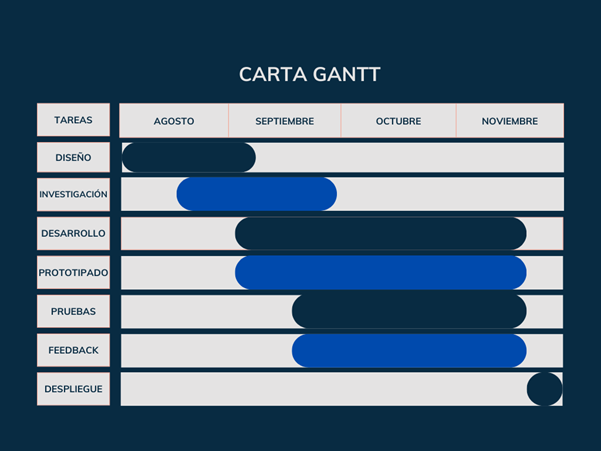
\includegraphics{gantt.png}
  \end{center}
  \caption[Carta Gantt del proyecto]{Carta Gantt del proyecto}
  \label{fig:gantt}
\end{figure}

\newpage

\subsection{Anexo Resumen de Esfuerzo}
\begin{center}
  \begin{tabular}{ | p{10cm} | p{5cm} |}
    \hline
    \multicolumn{1}{|c|}{\textbf{Actividad}} & \multicolumn{1}{|c|}{\textbf{Número de Horas}} \\
    \hline
    
    {Preparación del proyecto} & {20} \\ \hline
    {Desarrollo del módulo de autos} & {50} \\ \hline
    {Desarrollo del módulo de pistas} & {50} \\ \hline
    {Desarrollo del módulo de sesiones} & {80} \\ \hline
    {Desarrollo del módulo de temporadas} & {80} \\ \hline
    {Corrección de errores de código} & {40} \\ \hline
    {Despliegue de la aplicación} & {27} \\ \hline
    {Control de versiones} & {37} \\ \hline
    
    {\textbf{Total}} & {\textbf{384}} \\

    \hline
  \end{tabular}
  
    \captionof{table}{Tabla de resumen de esfuerzo}\label{table:effort}
\end{center}

\newpage

\section{Anexos Retrospectiva del Proyecto}

\subsection{Anexo Iteraciones en el Desarrollo}

\begin{center}
  \begin{tabular}{ | p{6cm} | p{3cm} | p {6cm} |}
    \hline
    \multicolumn{1}{|c|}{\textbf{Funcionalidad}} & \multicolumn{1}{|c|}{\textbf{Fecha}} &
    \multicolumn{1}{|c|}{\textbf{Retroalimentación}} \\
    \hline
    
    {Módulo de Autos (1)} & {12/11/2023} & {Añadir visualización para todos los autos y un sólo auto.}\\
    {Módulo de Autos (2)} & {12/11/2023} & {Agregar los autos tanto a la navegación como a la sub-navegación de la aplicación}\\
    {Módulo de Autos (3)} & {21/11/2023} & {Corregir problemas internos del modelo de autos}\\ \hline
   
    {Módulo de Pistas (1)} & {11/11/2023} & {Corregir problemas de validación en el modelo de Pista}\\
    {Módulo de Pistas (2)} & {12/11/2023} & {Agregaron las pistas tanto a la navegación como a la sub-navegación de la aplicación}\\
    {Módulo de Pistas (3)} & {28/11/2023} & {Mejorar la relación a modelos de Pista desde la visualización del modelo de Sesión.}\\ \hline
    
    {Módulo de Temporadas (1)} & {19/11/2023} & {Generar modelos de Ranking asociados a la temporada automáticamente después de crearla}\\
    {Módulo de Temporadas (2)} & {30/11/2023} & {Eliminar entradas de resultado de jugador asociadas a la temporada si estas tienen todos sus parámetros en cero}\\ \hline
    
    {Módulo de Sesiones (1)} & {19/11/2023} & {Determinar el número de cada sesión automáticamente una vez creada}\\
    {Módulo de Sesiones (2)} & {28/11/2023} & {Añadir botón de descarga para el Session Log asociado a cada sesión}\\
    {Módulo de Sesiones (3)} & {29/11/2023} & {Añadir acciones de administrador a la vista de sesión, tales como eliminar}\\
    
    \hline
  \end{tabular}
  
    \captionof{table}{Tabla de iteraciones en el desarrollo}\label{table:iterations}
\end{center}
